\begin{figure}[H]
\centering
\includegraphics[page=6,width=0.48\textwidth]{\FCNCFigures/xTFW/showFake/NOMINAL/reg2mtau1b2jos_vetobtagwp70_highmet/tau_pt_0.pdf}
\put(-100, 140){\textbf{(a1)}}
%\put(-120, 130){\footnotesize{$t_h\thadhad$-2j (OS)}}
\includegraphics[page=6,width=0.48\textwidth]{\FCNCFigures/xTFW/showFake/NOMINAL/reg2mtau1b3jos_vetobtagwp70_highmet/tau_pt_0.pdf}
\put(-100, 140){\textbf{(b1)}}
%\put(-120, 130){\footnotesize{$t_h\thadhad$-3j (OS)}}
\caption{ The distributions of $\tau$ $\pt$ in the $t_h\thadhad$-2j (a1), $t_h\thadhad$-3j (b1) using the nominal FFs.Only statistical uncertainties are being shown. Underflow and overflow bins are included respectively in the first and last bins. The real tau contributions shown from various MC samples. }
\label{fig:fakeEstimation_had_nominal}
\end{figure}

